% updated in April 2002 by Antje Endemann
% Based on CVPR 07 and LNCS, with modifications by DAF, AZ and elle, 2008 and AA, 2010, and CC, 2011; TT, 2014; AAS, 2016

\documentclass[runningheads]{llncs}
\usepackage{graphicx}
\usepackage{amsmath,amssymb} % define this before the line numbering.
\usepackage{color}
\usepackage{subfiles}
\usepackage[width=122mm,left=12mm,paperwidth=146mm,height=193mm,top=12mm,paperheight=217mm]{geometry}
\begin{document}
% \renewcommand\thelinenumber{\color[rgb]{0.2,0.5,0.8}\normalfont\sffamily\scriptsize\arabic{linenumber}\color[rgb]{0,0,0}}
% \renewcommand\makeLineNumber {\hss\thelinenumber\ \hspace{6mm} \rlap{\hskip\textwidth\ \hspace{6.5mm}\thelinenumber}}
% \linenumbers
\pagestyle{headings}
\mainmatter

\title{Penguin colony detection with deep learning.\\
\large Performance of U-Net as the amount of training data grows.
} % Replace with your title

\titlerunning{Technical Report}

\maketitle

%\begin{abstract}
%The abstract should summarize the contents of the paper. LNCS guidelines
%indicate it should be at least 70 and at most 150 words. It should be set in 9-point
%font size and should be inset 1.0~cm from the right and left margins.
%\dots
%\keywords{We would like to encourage you to list your keywords within
%the abstract section}
%\end{abstract}
\section{2nd-May-2018 | Exp: Performance of the model as the amount of training data grows.}

The experiments are conducted 3 times independently. For each trial, all data is randomly divided into 5 folds. The last chunk of data is kept untouched for testing. The first fold is used for training the first model. The first and second are used for training the second model. Likewise, the third model is trained on three chunk of data and the fourth model trained on four. Thus, from the first model to the fourth model, each is introduced with more training data. All other settings are the same for all models.

The results are shown in Figure \ref{fig:trend} and visualized in Figure \ref{fig:dgrow1} and Figure \ref{fig:dgrow2}  

\def\subFigx{0.8\linewidth}
\begin{figure}[h] 
\centering
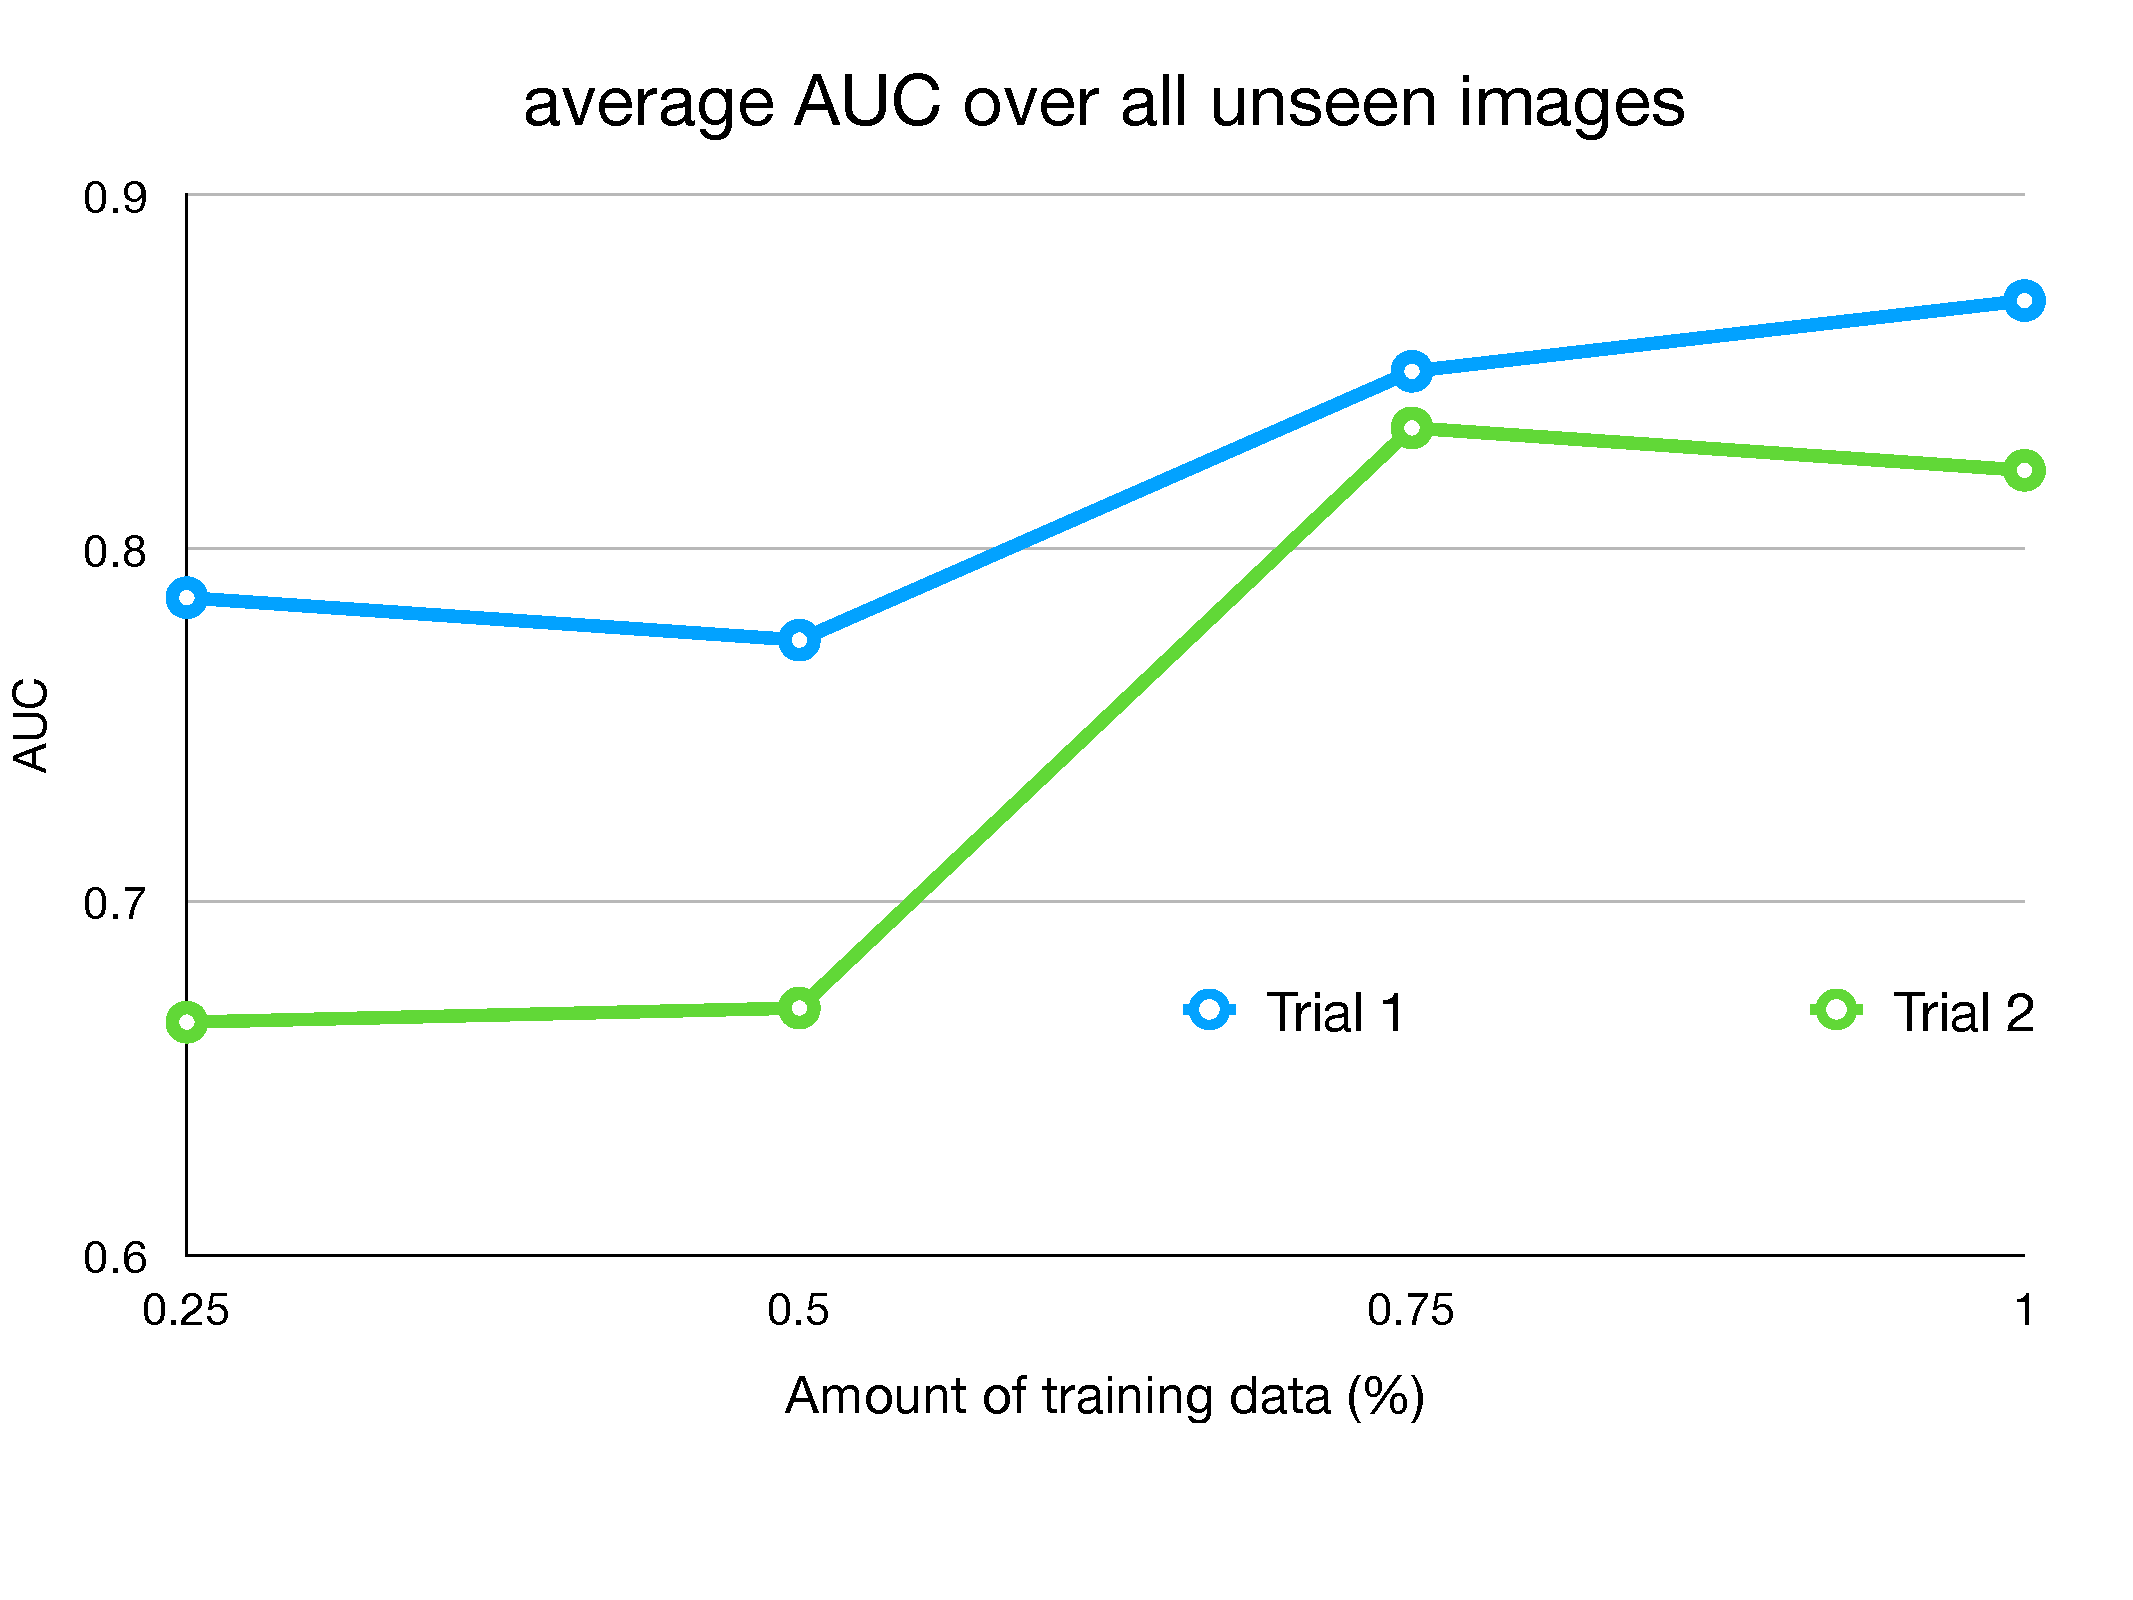
\includegraphics[width=\subFigx]{./fig/datagrow/keynote/datagrow_diagram.pdf}
\caption{{ Performance of U-Net with different amount of training data.}}
\label{fig:trend}
\end{figure}
\subfile{fig/datagrow}







\clearpage

\bibliographystyle{splncs03}
\bibliography{egbib}
\end{document}
